%
\documentclass[11pt]{thesis} % draft

\title{Algorithmic Meta-Creativity}
\author{Fania Raczinski}
\date{March 2015}


\begin{document}
\pagestyle{plain}

\tableofcontents

% !TEX root = ../test.tex

\chapter{One}

\startcontents[chapters]

\minicontents

\spirals

\section{Two}
\fbox{hello}
\lipsum[1]
\subsection{Three}
\lipsum[1]
\subsection{Three}
\lipsum[1]
\section{Two}
\lipsum[1]
\section{Two}
\lipsum[1]
\subsection{Three}
\section{Two}
\subsection{Three}
\section{Two}
\section{Two}

\stopcontents[chapters]

% !TEX root = ../test.tex

\chapter{One}

\startcontents[chapters]

\minicontents

\spirals

\section{Two}
\lipsum[1]
\subsection{Three}
\lipsum[1]
\subsection{Three}
\section{Two}
\lipsum[1]
\section{Two}


\stopcontents[chapters]
% % !TEX root = ../main.tex

\chapter{Methodology}
\label{ch:methodology}

\startcontents[chapters]

\vfill

\begin{alltt}\sffamily
Entire regions of our planetary system,
that great golden key with which you are playing,
and of the system of this Universe,
time to the necessity of performing this pilgrimage.
 
Would arrive at the correct solution,
face shews not the least wrinkle,
through his rash opinion of the improbability of performing,
faire ici le compte rendu technique de ma decouverte.

Acting upon this hint,
acted violently on my nervous system,
this was caused by intense heat acting on the organic matter of the earth.

The sum total of good playing,
and the Machine playing its large Wings,
that I would try it on myself acting forthwith on this decision.
\end{alltt}

\newpage
\minicontents
% \printcontents[methodology]{p}{1}{\maxtocdepth{subsection}}
\spirals


This project combines research in science, art and the humanities---making it transdisciplinary.

\begin{description}[leftmargin=3cm]
  \item [Pataphysics] Literature, Philosophy, Art
  \item [Creativity] Cognitive Science, \ac{AI}, \ac{DH}
  \item [Technology] \ac{IR}, \ac{NLP}, Web Development
\end{description}

Traditional methodologies in these disciplines are very subject specific and a project combining elements of each field is left mixing and matching suitable methods from them all.

In this chapter I will outline the reasons why the existing intradisciplinary methodologies aren't completely suitable for this project and then explain the choice of more transdisciplinary methods and how I combined them to suit my needs.

As mentioned in the~\nameref{ch:introduction}\sidepar{§~\ref{s:intromethod}} the overall objectives of this project are to:

\label{s:objectives}
\begin{enumerate}
  \item Critically analyse and synthesise existing literature,\sidepar{\textspiral~\ref{p:lit}}
  \item develop pataphysical algorithms,\sidepar{\textspiral~\ref{p:practice}}
  \item design a system to demonstrate algorithms,\sidepar{\textspiral~\ref{p:practice}}
  \item develop a website as an artefact,\sidepar{\textspiral~\ref{p:practice}}
  \item define an evaluation and interpretation framework,\sidepar{\textspiral~\ref{p:theory}}
  \item analyse results.\sidepar{\textspiral~\ref{p:analysis}}
\end{enumerate}

Research methods that support these tasks are needed and I will address these four points again at the end of this chapter\sidepar{§~\ref{s:mymeth}}.


\section{Intradisciplinary}

Different disciplines prefer different research methodologies. Of the various disciplines that inform this research the specific subareas that are relevant are as follows.

\begin{itemize}
  \item Information Retrieval
  \item Interface Design
  \item Web Development
  \item Poetry, Literature, and Art
  \item Philosophy
  \item Human and Machine Creativity
  \item Creative Computing
  \item Computational Creativity
\end{itemize}


\subsection{Technology}

Half of this project's objectives are related to computer science therefore it is important to consider how research in this discipline is traditionally approached.

A framework for finding a suitable approach was suggested by Holz et al \autocite*{Holz2006}. The following four steps form an iterative process. (1) ``What do we want to achieve?'' e.g. find out what is happening, develop something that works, evaluate an existing system/technology, compare existing systems, or change human behaviour. (2) ``Where does the data come from?'' e.g. how to collect? (read, observe, ask, measure, experiment, model) and where to collect? (field, laboratory, conceptual). (3) ``What do we do with the data?'', e.g. identify themes/patterns/quotes, calculate numbers, identify trends, express via multimedia, create frameworks/taxonomies. (4) ``Have we achieved our goal?'' e.g. draw conclusions, evaluate results, or identify limitations.

Another option is to look at what computer science researchers have done historically. In a rather old but still insightful analysis of over 600 papers\footnote{While the paper itself was published in 2004, the body of work was based on publications from between 1995 and 1999---this suggests that a lot of the more ``recent'' research around web technologies is not included in this study.} Ramesh et al \autocite*{Ramesh2004} have shown that---by far---the most common approach to research in computer science during this period was \emph{formulative} with almost 79\% use (as opposed to ``descriptive'' with 10\% and ``evaluative'' with 11\%). This was in particular in regards to ``processes, methods and algorithms'' which was used by just over 50\% of researchers. Not surprisingly the most popular research method was \emph{mathematical conceptual analysis} with about 75\% use.

Jose Nelson Amaral \autocite*{Amaral2006} classifies methodologies in computer science into five main categories as shown below.

\begin{description}[leftmargin=3.5cm]
  \item [Formal] Proof, verification, correctness
  \item [Experimental] Testing, evaluation, question answering
  \item [Build] Proof of concept, prototype, artefact
  \item [Process] Understand and define processes
  \item [Model] Abstraction, simulations
\end{description}

\spirals

Here are this project's answers to the four questions posed by Holz et al \autocite*{Holz2006}.

\begin{description}
  \item[What do we want to achieve?]~
    - Understand human creativity and how this translates to machines.\\
    - Understand the relationship of pataphysics and creativity.\\
    - Understand how creativity is evaluated in humans and machines.\\
    - Research suitable pataphysical concepts to be implemented as algorithms.\\ 
    - Define algorithms formally.\\
    - Implement prototype incorporating algorithms.\\
    - Develop framework for interpreting and evaluating machine creativity.
	\item[Where does the data come from?]~
    - Read pataphysical literature and research.\\
    - Collate existing research on creativity and evaluation.\\
    - Survey creative approaches to technology.\\
    - Experiment with algorithms and implementation.
	\item[What do we do with the data?]~
    - Iterate through developmental stages of algorithmic outputs.\\
    - Create an artefact that represents the underlying philosophy and research.\\
    - Create an evaluation framework based on theoretical research.
  \item[Have we achieved our goal?]~
    - See conclusion chapter~\ref{ch:observations}\sidepar{§~\ref{ch:observations}}.
\end{description}

Referring back to the four objectives above (see page~\pageref{s:objectives}), objective 1 is to create new creative search algorithms. This is not supposed to happen on a purely abstract basis but in a practical fashion (i.e. `experimental'), with a working implementation (i.e. `build') as proof-of-concept (see objective 2). While the algorithms need to be defined in formal terms (i.e. `formal'), the goal here is not to create a theoretical proof of correctness (given the creative and rather subjective nature of the underlying philosophy this is virtually impossible) but a practical demonstration of the creative processes behind. Overall this would suggest an experimental approach with prototyping of an artefact. Objective \num{3} is to come up with a suitable definition of creativity (i.e. `process'). This should be informed by existing research. Again, we are not interested in formulating this in mathematical terms and proofs but rather a more esoteric and systemic view. Because the definition needs to apply to humans and machines it needs to be precise enough. Objective \num{4} is then to create an overall theoretical framework (i.e. `model') for the evaluation of creativity in humans and machines.

By now we have managed to cover every one of the major methodologies mentioned by Amaral et al. \autocite*{Amaral2006} but we are still lacking ways to address the subjective and creative nature of the project. Furthermore, the philosophical and artistic inspirations that inform the development of the artefact don't get enough of a voice in these methods. In computer science, implementations are generally seen as a proof of concepts or prototypes---when really they should be seen as artefacts in the sense of artistic pieces of work. So, to really appreciate the scope of this practical element of this project we need to consider research in the arts and humanities too.


\subsection{Arts and Humanities}

% \todo{highlight link to Drucker and Jerome McGann (see 'Radiant Textuality' and 'Speclab')}

\begin{quotation}
  A hallmark of humanistic study is that research is approached differently than in the natural and social sciences, where data and hard evidence are required to draw conclusions. Because the human experience cannot be adequately captured by facts and figures alone, humanities research employs methods that are historical, interpretive and analytical in nature. \sourceatright{\autocite{Standford2016}}
\end{quotation}

Malins and Gray suggest the following ideas for arts-based researchers searching for the right methodology \autocite*{Malins1995}.

\begin{itemize}
  \item Consider a range of research strategies (from all disciplines).
  \item `Tailor' the research to the nature of project and the researcher's expertise.
  \item Carry out the research from an informed perspective, as `participant observer'.
  \item Continually define and refine the research question, allowing methodologies to emerge.
  \item Acknowledge accessibility, discipline, rigour, transparency, and transferability.
  \item Be aware of the critical context of practice and research and raise the level of critical debate.
  \item Consider interdisciplinary / multidisciplinary approaches to research.
\end{itemize}

They further elaborate on the key characteristics of arts methodologies as follows \autocite{Gray2004}.

\begin{quotation}
\begin{itemize}
  \item Experiencing/exploring, gathering, documenting information and generating data/evidence.
  \item Reflecting on and evaluating information, selecting the most relevant information.
  \item Analysing, interpreting and making sense of information.
  \item Synthesizing and communicating research findings, planning new research.
\end{itemize}\sourceatright{\autocite{Gray2004}}
\end{quotation}

They further specify a whole set of individual methods used for the approaches above.

\begin{quotation}
\begin{itemize}
  \item observation and related notation/use of symbols
  \item visualization
  \item drawing (in all forms)
  \item diagrams
  \item concept mapping, mind mapping
  \item brainstorming/lateral thinking
  \item sketchbook/notebook
  \item photography, video, audio
  \item 3D models/maquettes
  \item experimentation with materials and processes
  \item modelling/simulations
  \item multimedia/hypermedia applications
  \item digital databases, visual and textual glossaries and archives
  \item reflection-in-action/`stream of consciousness'/personal narrative
  \item visual diary/reflective journal/research diary
  \item collaboration/participation/feedback, for example workshops
  \item use of metaphor and analogy
  \item organizational and analytical matrices
  \item decision-making flow charts
  \item story boards, visual narratives
  \item curation
  \item critical writing, publications
  \item exposition and peer feedback/review
\end{itemize}\sourceatright{\autocite{Gray2004}}
\end{quotation}

The discpiline of \acf{DH} (see chapter~\ref{s:digithuman}\sidepar{§~\ref{s:digithuman}}) seems like a logical choice to look for suitable methodologies. It is characterised by ``collaboration, transdisciplinarity and an engagement with computing'' \autocite{Burdick2012} but it should not simply be reduced to ``doing the humanities digitally'' \autocite*{Burdick2012}. Transliteracy, an understanding of several kinds of tools and media, is an important aspect in this \autocite{Thomas2007}. \ac{DH} can be broken down into the following set of methodologies.

\begin{description}
  \item [Design] shape, scheme, inform, experience, position, narrate,
  					interpret, remap/reframe, reveal, deconstruct, reconstruct,
  					situate, critique
  \item [Curation, analysis, editing, modelling] digitise, classify, describe, metadata, organise, navigate
  \item [Computation, processing] disambiguate, encode, structure, procedure, index, automate, sort, search, calculate, match
  \item [Networks, infrastructure] cultural, institutional, technical, compatible, interoperable, flexible, mutable, extensible
  \item [Versioning, prototyping, failures]	iterate, experiment, take-risks, redefine, beta-test
\end{description}

Some of the emerging research methods Burdick et al. have identified are listed below \autocite*{Burdick2012} (The full list can be found in appendix~\ref{s:dhmap}\sidepar{§~\ref{s:dhmap}}).

\begin{multicols}{2}\raggedright
\begin{itemize}
  \item structured mark-up
  \item	natural language processing
  \item	mutability
  \item	digital cultural record
  \item	algorithmic analysis
  \item distant/close, macro/micro, surface/depth
  \item parametrics
  \item	cultural mash-ups
  \item	algorithm design
  \item data visualization
  \item	modelling knowledge
  \item	ambient data
  \item	collaborative authorship
  \item	interdisciplinary teams
  \item	use as performance
  \item narrative structures
  \item	code as text
  \item	software in a cultural context
  \item repurposable content and remix culture
  \item participatory web
  \item	read/write/rewrite
  \item	meta-medium
  \item	polymorphous browsing
\end{itemize}
\end{multicols}

\spirals

Several of the methodologies listed by Gray and Malins \autocite*{Gray2004} seem to apply to the research presented in this thesis. Exploring, evaluating, analysing, interpreting, synthesising and disseminating research all are part of it. However, looking at the specific methods they collated, the difference becomes clearer as only the following 7 appear relevant (visualization, experimentation with processes, multimedia/hypermedia applications, use of metaphor and analogy, organizational and analytical matrices, curation, and critical writing, publications).

The \ac{DH} methodologies seem more useful. In terms of \textbf{design}, \url{pata.physics.wtf} \textit{positions} itself in context and the evaluation framework \textit{interprets} and \textit{critiques} \ac{AMC}. Before that I \textbf{curate} the two corpora, \textit{digitise} them and \textit{organise} them. \textbf{Computing} comes in at verious stages, to \textit{(dis)ambiguate} (i.e. pataphysicalise), \textit{encode}, \textit{index}, \textit{search} and \textit{match} data. The \textbf{infrastructure} is \textit{cultural}, \textit{technical} and \textit{extensible}, relying on the \ac{WWW} for several spects. \textbf{Versioning, prototyping and failures} all come in during the \textit{iterative} development process, which involves a lot of \textit{experimentation} and refactoring. Furthermore, the research methods Burdick et al \autocite*{Burdick2012} list match this project much better (although of course the list above was already only a selection that was deemed relevant; the original list was much larger. See appendix~\ref{s:dhmap}\sidepar{§~\ref{s:dhmap}}).


\section{Transdisciplinary}

Nicolescu distinguished between 3 different kinds of research ``without stable boundaries between the disciplines''.\footnote{Nicolescu cites Jean Piaget here, who first coined the term `transdisciplinarity' in 1972.} \autocite*{Nicolescu2010}.

\begin{description}
  \item [Multidisciplinarity]	concerns itself with studying a research topic in not just one discipline but in several simultaneously.
  \item [Interdisciplinarity]	concerns the transfer of methods from one discipline to another.
  \item [Transdisciplinarity]	concerns that which is at once between the disciplines, across the different disciplines, and beyond all disciplines.
\end{description}

The standard epistemological view of science and art is that they are objective and subjective, respectively. So, what does that mean for research conducted between, across and beyond science and art, i.e. research that is transdisciplinary?

Nicolescu criticised the view that science must be objective. He even claimed that any non-scientific knowledge is ``cast into the inferno of subjectivity, tolerated at most as a meaningless embellishment or rejected with contempt as a fantasy, an illusion, a regression, or a product of the imagination'' \autocite*{Nicolescu2010}. Objectivity, he said, becomes the ``supreme criterion of Truth''\footnote{As we shall see later, pataphysics does the opposite: it reveres the Subject.}

\begin{quotation}
  The death of the Subject is the price we pay for objective knowledge. \sourceatright{\autocite{Nicolescu2010}}
\end{quotation}

He went on to quote Werner Heisenberg on the concepts of objective and subjective reality: ``we would make a very crude simplification if we want to divide the world in[to] one objective reality and one subjective reality. Many rigidities of the philosophy of the last centuries are born by this black and white view of the world'' \autocite[Heisenberg, cited in][]{Nicolescu2010}.

\begin{quotation}
  The too strong insistence on the difference between scientific knowledge and artistic knowledge comes from the wrong idea that concepts describe perfectly the `real things'. [\ldots] All true philosophy is situated on the threshold between science and poetry. \sourceatright{\autocite[Heisenberg, cited in][]{Nicolescu2010}} \footnote{The full paragraph is worth quoting---see appendix~\ref{s:heisenberg}.}
\end{quotation}

In transdisciplinarity traditional disciplinary boundaries have no meaning.

\begin{figure}[!htbp]
\centering
  \begin{tikzpicture}
    \node [box] at (1.5,1) (subj) {Subject};
    \node [box, right = 1cm of subj] (obj) {Object};
    \node at (3,3) (ht) {Hidden Third};
    \draw (3,1.75) circle [radius=3cm]; 
    \node at (6.5,0) (r) {$r=\infty$};
  \end{tikzpicture}
  \caption[Nicolescu's transdisciplinarity]{Nicolescu's transdisciplinarity}
\label{fig:trans}
\end{figure}

Working across disciplines requires a new unique methodology. Nicolescu proposed a methodology of transdisciplinarity as a non-hierarchical ternary partition of `Subject, Object and Hidden Third' (as shown in figure~\ref{fig:trans}\sidepar{\faicon{object-group}~\ref{fig:trans}}) rather than the traditional binary partition of `Subject versus Object' \autocite*{Nicolescu2010}.

\begin{quotation}
  The old principle ``unity in diversity and diversity from unity'' is embodied in transdisciplinarity.' \sourceatright{\autocite{Nicolescu2010}}
\end{quotation}

\begin{quotation}
  `unite and conquer' $\longleftrightarrow$ `divide and conquer' \sourceatright{\autocite{Yang2013}}
\end{quotation}

Hugill and Yang agree that existing research methodologies are unsuitable for transdisciplinary subjects such as \acf{CC}. The following is an example of a possible \ac{CC} research methodology they propose as a starting point \autocite{Hugill2013c}:

\begin{enumerate}
  \item Review literature across disciplines.
  \item Identify key creative activities.
  \item Analyse the processes of creation.
  \item Propose approaches to support these activities and processes.
  \item Design and implement software following this approach.
  \item Experiment with the resulting system and propose framework.
\end{enumerate}

They go on to propose four standards for \ac{CC} \autocite{Hugill2013c} namely, (1) resist standardisation, (2) perpetual novelty, (3) continuous user interaction and (4) combinational, exploratory and or transformational.

A different model was suggested by Edmonds and Candy in their \ac{TMPR}, a framework to ``influence practice, inform theory and, in particular, shape evaluation'' \autocite*{Edmonds2010}. Figure~\ref{fig:tmpr}\sidepar{\faicon{object-group}~\ref{fig:tmpr}} shows the \ac{TMPR} which allows for different trajectories between practice, theory and evaluation. Table~\ref{tab:tmpr}\sidepar{\faicon{table}~\ref{tab:tmpr}} shows the various elements, activities and outcomes in this framework more clearly.

\begin{figure}[!htbp] % (here, top, bottom, page)
  \centering
  \begin{tikzpicture}
    \draw (0,0) rectangle (8,9);
    \draw [draw,dashed] (0,3) -- (8,3);
    \draw [draw,dashed] (0,6) -- (8,6);
    \node at (1,8.5) (p) {Practice};
    \node at (1,5.5) (t) {Theory};
    \node at (1.3,2.5) (e) {Evaluation};
    \node [box] at (4.5,1.5) (results) {Results};
    \node [box] at (2.5,4.5) (criteria) {Criteria};
    \node [box] at (6.5,4.5) (frameworks) {Frameworks};
    \node [box] at (4.5,7.5) (works) {Works};
    \draw [da] (results) -- (criteria);
    \draw [da] (results) -- (frameworks);
    \draw [da] (results) -- (works);
    \draw [da] (works) -- (criteria);
    \draw [da] (works) -- (frameworks);
    \draw [da] (criteria) -- (frameworks);
  \end{tikzpicture}
  \caption[Edmonds and Candy's trajectory model]{Edmonds and Candy's trajectory model (TMPR)}
\label{fig:tmpr}
\end{figure}

\begin{table}[!htbp]
\caption[Elements, activities and outcomes of the TMPR]{Elements, activities and outcomes of each trajectory in the TMPR}
\label{tab:tmpr}
  \begin{tabu}{X[1]X[2]X[3]}
  \toprule
  \textbf{Elements}
  &
  \textbf{Activities}
  &
  \textbf{Outcomes}
  \\ \midrule
  \textbf{Practice}
  &
  create, exhibit, reflect
  &
  \textbf{Works:} consisting of physical artefacts, musical compositions, software systems, installations, exhibitions, collaborations
  \\ \midrule
  \textbf{Theory}
  &
  read, think, write, develop
  &
  \textbf{Frameworks:} comprising questions, criteria, issues
  \\ \midrule
  \textbf{Evaluation}
  &
  observe, record, analyse, reflect
  &
  \textbf{Results:} findings leading to new/modified Works and Frameworks
  \\ \bottomrule
  \end{tabu}
\end{table}

\spirals

This project positions itself ``at once between the disciplines, across the different disciplines, and beyond all disciplines''---making it transdisciplinary. The abolishment of disciplinary boundaries suits the unique context of this research. Pataphysics specifically is highly subjective. Searle highlighted that ontologically subjective topics (such as creativity) can be studied in epistemically objective ways \autocite*{Searle2015}, which, as doctoral research, this project attempts to do.

The Hugill and Yang \ac{CC} methodology seems general enough to fit the needs of this project, with all 6 points covered in the various chapters of this thesis.

\begin{enumerate}
  \item Review literature across disciplines (chapters~\ref{ch:inspirations}, \ref{ch:pataphysics}, \ref{ch:creativity}, \ref{ch:technology}, and \ref{ch:evaluation}).
  \item Define creativity in humans and machines (chapters~\ref{ch:pataphysics},~\ref{ch:creativity},~\ref{ch:technology} and \ref{ch:evaluation}).
  \item Analyse the relation between the disciplines above (chapter~\ref{ch:foundations}).
  \item Propose algorithms to support creativity in machines (chapter~\ref{ch:implementation}).
  \item Design and implement software following this approach (chapter~\ref{ch:implementation}).
  \item Experiment with the resulting system and propose interpretation/evaluation framework (chapters~\ref{ch:analysis}, \ref{ch:future}, and \ref{ch:interpretation}).
\end{enumerate}

Figure~\ref{fig:ftmpr}\sidepar{\faicon{object-group}~\ref{fig:ftmpr}} on page~\pageref{fig:ftmpr} shows how the \ac{TMPR} could be applied to this project. 


\section{Patadisciplinary}
\label{s:mymeth}

So, to summarise, this project draws from several different disciplines as mentioned at the beginning of this chapter (page~\pageref{ch:methodology}): pataphysics---literture, philosophy, art, creativity---cognitive science, \ac{AI}, \ac{DH}, and technology---\ac{IR}, \ac{NLP}, web development.

\begin{description}[leftmargin=3.2cm]
  \item [Epistemology] Transdisciplinary, subjective
  \item [Methodology] Creative computing, exploratory, experimental
  \item [Methods] Artefact, literature synthesis, algorithm design, theoretical framework, critical reflection and analysis, rapid incremental prototyping
\end{description}

The general workflow of this project was as follows: (1) critically analyse and synthesise existing literature, (2) develop pataphysical algorithms, (3) design a system to demonstrate algorithms, (4) develop a website as an artefact, (5) define an evaluation and interpretation framework, and (6) analyse results.

\begin{figure}[!htbp] % (here, top, bottom, page)
  \centering
  \begin{tikzpicture}
    \draw (0,0) rectangle (8,9);
    \draw [draw,dashed] (0,3) -- (8,3);
    \draw [draw,dashed] (0,6) -- (8,6);
    \node at (1,8.5) (p) {Practice};
    \node at (1,5.5) (t) {Theory};
    \node at (1.2,2.5) (e) {Evaluation};
    \node [box] at (4.5,1.5) (results) {Results};
    \node [box] at (2.5,4.5) (criteria) {Criteria};
    \node [box] at (6.5,4.5) (frameworks) {Frameworks};
    \node [box] at (4.5,7.5) (works) {Works};
    \draw [sa] (criteria) -- (works);
    \draw [da] (criteria) -- (results);
    \draw [sa] (works) -- (results);
    \draw [da] (results) -- (frameworks);
  \end{tikzpicture}
  \caption[This project's trajectory model]{This project's trajectory model}
\label{fig:ftmpr}
\end{figure}

As figure~\ref{fig:ftmpr}\sidepar{\faicon{object-group}~\ref{fig:ftmpr}} shows, the practive trajectory of this research is based on the practical development of a website to contain the exploratory search tool and implementation of the theoreical algorithms. The theory trajectory is about defining those algorithms formally in historic and topical context based on a critical survey of related literature. This also includes the development of a theoretical framework for the evaluation and interpretation of creative artefacts. The Evaluation trajectory then is all about the results. That includes an analysis of the work completed. The arrows in the figure indicate how these different trajectories influence each other.


\stopcontents[chapters]


\phantomsection
\addtocontents{toc}{\protect\vspace{20pt}}
\addcontentsline{toc}{part}{HELLO WORLD}
\partimage[width=\textwidth]{spiral_hello.pdf}
\part{\texorpdfstring{H\scalebox{2.2}{$\boldsymbol\Sigma$}LL\scalebox{2.2}{$\boldsymbol\Theta$} W\scalebox{2.2}{$\boldsymbol\Theta$}RLD}{HELLO WORLD}}
% % !TEX root = ../main.tex

\chapter{Introduction}
\label{ch:introduction}

\startcontents[chapters]

\vfill

\begin{alltt}\sffamily
Feeling a movement of pity,
discovered the induction coil,
cette irraisonnee induction,
and entered the opening in the wall.

Only by some recherche movement,
apres coup et sous forme d'introduction,
opening his seized manuscript,
the enemy made within the enclosure of the vineyard.

Which he had thrown off at the beginning of his labor,
in opening so exactly at the,
than the thirst of my paternity.

We can then start at once,
and whose informing voice had consigned me to the hangman,
as any person at all conversant with authorship may satisfy himself at.
\end{alltt}

\newpage
% {\Large\sffamily\scshape\textbf{1.0 \quad Introduction Contents}}
% \vspace{0.5cm}
\minicontents
\spirals

This thesis describes \acf{AMC}. In other words it is about using creative computing to achieve computer creativity.

The project is transdisciplinary;\marginpar{§~\ref{ch:methodology}} it is heavily inspired by the absurd French pseudo-philosophy pataphysics\marginpar{§~\ref{ch:pataphysics}} and draws from a wide range of subject areas such as computer science, psychology, linguistics, literature, art and poetry, languages and mathematics.

The research\marginpar{§~\ref{ch:foundations}} included exploring what it means to be creative as a human, how this translates to machines, how pataphysics relates to creativity and how creativity should be evaluated in machines\marginpar{§~\ref{ch:interpretation}}.

Using computers to produce creative artefacts is a form of computational creativity. Using creative techniques computationally is creative computing. \ac{AMC} spans the two---whether this is to achieve a creative or non-creative output. It is the use of digital tools (which may not be creative themselves) and the way they are used forms the creative process or product. 

Creativity in humans needs to be interpreted differently to machines\marginpar{§~\ref{s:theoryanalysis}}. Humans and machines differ in many ways, we have different `brains/memory', `thinking processes/software' and `bodies/hardware'. Too often creative output by machines is judged as we would a human's. 

Computers which are truly artificially intelligent might be capable of true artificial creativity. Until then they are (philosophical) zombie robots: machines that behave like humans but aren't conscious. The only alternative is to see any computer creativity as a direct or indirect expression of human creativity using digital means and evaluate it as such. \ac{AMC} is neither machine creativity nor human creativity---it is both. By acknowledging the undeniable link between computer creativity and its human influence (the machine is just a tool for the human) we enter a new realm of thought. How is \ac{AMC} defined and evaluated? This thesis addresses this issue. 

\begin{enumerate}
  \item a practical demonstration of \ac{AMC}
  \item a theoretical framework to help interpret and evaluate products of \ac{AMC}
\end{enumerate}

The outcome of step (1)\marginpar{§~\ref{ch:implementation}} is presented as a website---\url{pata.physics.wtf}---written in \num{5} different programming languages\footnote{Python, \acs{HTML}, \acs{CSS}, Jinja, JavaScript}, making calls to \num{6} external web services\footnote{Microsoft Translate, WordNet, Bing, Getty, Flickr and YouTube}, in a total of over \num{3000} lines of code\footnote{\num{2864} lines of code, \num{489} lines of comments - as of 08 Dec 2015} spread over \num{30} files.

The main purpose of the system above is to demonstrate the three creative \emph{patalgorithms} in the context of exploratory \acf{IR}\marginpar{§~\ref{s:algorithms}}. A browsing rather than a search engine, it presents results in various formats such as sonnets and golden spirals. The system partially automates the creative process, generating results on demand, which allows users to focus on their own personal artistic evaluation rather than production.

Immediate inspirations\marginpar{§~\ref{ch:inspirations}} come from fictional character \textit{Doctor Faustroll} created by French absurdist and `father' of pataphysics Alfred Jarry \autocite*{Jarry1996}, the fantastic taxonomy of the \textit{Celestial Emporium of Benevolent Knowledge} by magical realist Jorge Luis Borges \autocite*{Borges2000} and \textit{A Hundred Thousand Billion Poems} by pataphysician and Oulipo co-founder Raymond Queneau \autocite*{Queneau1961}, amongst others.

To address step (2) above, I explored the problem of objective evaluation and interpretation\marginpar{§~\ref{ch:interpretation}} of subjective creativity specifically in regards to \ac{AMC}. I have argued that the most appropriate way to approach this is by looking at five objective constraints (person, process, product, place, purpose) and seven subjective criteria (novelty, value, quality, purpose, spatial, temporal, ephemeral) holistically and by understanding that humour and art `lie in the ear and eye of the beholder'.

This resulted in an \emph{interpretation framework}\marginpar{§~\ref{s:framework}} visualised as an evaluation matrix (\num{5} constraints x \num{7} criteria)\marginpar{\faicon{object-group}~\ref{fig:matrix}} which can be used to qualitatively and/or quantitatively measure the creativity of a given \ac{AMC} artefact:

\begin{enumerate}
  \item a set of scales that can be used to approximate a `rating' for the creative value of an artefact,\marginpar{§~\ref{s:sec}}
  \item a set of criteria to be considered using the scales above,\marginpar{§~\ref{s:oec}}
  \item a combined framework for evaluation.\marginpar{§~\ref{s:framework}}
\end{enumerate}


\section{Motivation}

Computers\marginpar{§~\ref{ch:technology}} are binary machines; the world is black and white to them (0 and 1, on and off). Programmers can run abstract high-level commands which are executed in sequence (with fast speeds giving the illusion of multitasking). They are precise, structured, logical, and generally abide by strict standards. Computers can only be creative if they are given clear instructions as to how. \acl{IR} is generally focused on relevance of results in regards to the query.

\begin{quotation}
  The Analytical Engine has no pretensions whatever to \emph{originate} anything. It can do \emph{whatever we know how to order it} to perform. \sourceatright{\autocite[Ada Lovelace, in][her emphasis]{Menabrea1842}}
\end{quotation}

Pataphysics\marginpar{§~\ref{ch:pataphysics}} emerged during the \textit{Belle Époque}\footnote{1871---1914} in France and has either directly or indirectly influenced various artistic movements such as Dada, Symbolism, Surrealism, Oulipo and Absurdist Theatre. Pataphysics is highly subjective and particular, values exceptions, the imaginary and the mutually incompatible.

Creativity\marginpar{§~\ref{ch:creativity}} is often studied at various levels (neurological, cognitive, and holistic/systemic), from different perspectives (subjective and objective) and characteristics (combinational, exploratory and transformative). It is usually defined in terms of value, originality and skill.

Combining computing with pataphysics seems impossible---although the antinomies below (juxtaposing principles in computing on the left with ideas from pataphysics on the right) highlight just how intriguing a possible combination of the two would be.

\begin{itemize}
  \item Polymorphism (generalisation) opposes particularity.
  \item Precision opposes exceptions and contradictions.
  \item Logic and structure oppose the imaginary and paradox.
  \item Cross-compatibility opposes the mutually exclusive.
  \item Responsiveness opposes the specific.
  \item Relevance opposes the creative.
\end{itemize}

This apparent dichotomy of computing and pataphysics is alluring. Christian B{\"o}k argued that pataphysics ``sets the parameters for the contemporary relationship between science and poetry'' \autocite*{Bok2002}. Pataphysics suddenly seems like the perfect choice infusing computers (science) with creativity (poetry).

Combining pataphysics with creativity\marginpar{\faicon{table}~\ref{tab:creatpata}} is easier. The ideas of combinatorial, exploratory and transformative creativity map quite nicely onto some pataphysical concepts such as clinamen, syzygy, antinomy and anomaly. 

Another motivating factor for this project was the lack of research in the particular area of creative computing\marginpar{§~\ref{ch:creativity}} in general. The discipline of computational creativity has emerged fairly recently\footnote{The first International Conferences on Computational Creativity ran in 2010 for example.} from a background in \ac{AI}. It appears to focus a lot more on the outcome of a product that would be judged creative rather than the actual process. Creative computing focuses on producing creative algorithms which may or may not have creative outputs. This was first addressed in \autocite{Raczinski2013}\marginpar{§~\ref{s:dc243article}} and later expanded into a definite description of this new discipline \autocite{Hugill2013c}.

\spirals

My personal interest in this project comes from a background in computer science and a longstanding interest in art. Most recently I managed to successfully combine my technical skills with my creative side for a Master of Science degree in Creative Technologies at \ac{DMU}\footnote{A passive interactive installation, augmenting a live video stream of users with interactive elements using motion tracking algorithms. See \url{msc.fania.eu} \autocite{Raczinski2010}.}. 


\section{Questions}

Research dealing with subjective ideas and concepts like creativity throws up a lot of questions. My intention is to address them all throughout this thesis, although some of them will not have definite binary answers. An attempt to answer them can be found in the conclusion chapter~\ref{s:answers}\marginpar{§~\ref{s:answers}}.

\begin{itemize}
  \item What is the relationship between pataphysics and creativity?
  \item How is computer creativity related to \ac{AI}?
  \item Should we distinguish between computationally automated or emulated creative processes and the programmer's input?
  \item How can a machine's creative output be evaluated?
  \item How can \ac{IR} be infused with creativity?
\end{itemize}


\section{Methodology}
\label{s:intromethod}

This project combines research\marginpar{§~\ref{ch:methodology}} in science and art making it transdisciplinary.

\begin{description}[leftmargin=3cm]
  \item [Pataphysics] Literature, Philosophy, Art, Poetry
  \item [Creativity] Cognitive Science, \ac{AI}, \ac{DH}
  \item [Technology] \ac{IR}, \ac{NLP}, Web Development
\end{description}

\begin{description}[leftmargin=3cm]
  \item [Epistemology] Transdisciplinary, subjective
  \item [Methodology] Creative computing, exploratory, experimental
  \item [Methods] Artefact, literature synthesis, algorithm design, theoretical framework, critical reflection and analysis, rapid incremental prototyping
\end{description}

The general process of my project was as follows.

\begin{enumerate}
  \item Critically analyse and synthesise existing literature,\marginpar{\textspiral~\ref{p:lit}}
  \item develop pataphysical algorithms,\marginpar{\textspiral~\ref{p:practice}}
  \item design a system to demonstrate algorithms,\marginpar{\textspiral~\ref{p:practice}}
  \item develop a website as an artefact,\marginpar{\textspiral~\ref{p:practice}}
  \item define an evaluation and interpretation framework,\marginpar{\textspiral~\ref{p:theory}}
  \item analyse results.\marginpar{\textspiral~\ref{p:analysis}}
\end{enumerate}


\section{Contributions}

The key contributions to knowledge described in this thesis are:

\begin{itemize}
  \item Three pataphysical search algorithms (clinamen, syzygy and antinomy).
  \item A creative exploratory search tool demonstrating the algorithms \url{pata.physics.wtf}.
  \item A set of 7 subjective criteria and 5 objective constraints for defining creativity.
  \item A combined framework for evaluating and interpreting creativity.
\end{itemize}


\section{Publications}

Some chapters (especially \nameref{ch:foundations} and \nameref{ch:interpretation})\marginpar{§~\ref{ch:foundations} \& \ref{ch:interpretation}} in this thesis are based partially on articles published during this project. I have used fragments from those papers freely without specific citations unless clearly indicated. I had several co-authors (Hongji Yang, Andrew Hugill, James Sawle and Dave Everitt) for these pieces and I hereby acknowledge their contributions.

A list of publications can be found in the preface on page~\pageref{pre:pub}. Details of talks and exhibitions and copies of the publications can be found in appendix~\ref{app:pub}\marginpar{§~\ref{app:pub}}.


\section{The Hitchhiker's Guide to this Thesis}

This document is organised into \num{6} parts which form the main logical structure of the thesis and each part contains several chapters. There are margin notes pointing to relevant chapters, sections, tables, figures or images throughout.


\subsection{Chapter Overview}

The preface contains the abstract, acknowledgments, and various tables of contents.

\begin{description}[leftmargin=3.5cm]
  \item[Introduction] Gives a general top-level overview of this research.
  \item[Inspirations] Lists the various immediate inspirations for the project.
  \item[Methodology] Explains and justifies the approach taken for the research.
  \item[Pataphysics] Describes the origins of pataphysics and related concepts. 
  \item[Creativity] Lists the theories of human and computer creativity.
  \item[Technology] Provides the technical background of this research.
  \item[Evaluation] Explains the models of evaluation for computer creativity.
  \item[Foundations] Brings together the research on creativity and pataphysics.
  \item[Interpretation] Critiques evaluation models and proposes a new approach.
  \item[Implementation] Describes \url{pata.physics.wtf} from a technical standpoint.
  \item[Applications] Showcases two use cases of this research.
  \item[Patanalysis] Analyses the artefact and some of the theoretical aspects. 
  \item[Asprirations] Addesses future work and known issues.
  \item[Outroduction] Summarises the contributions of this thesis.
\end{description}

The appendix contains additional material that was not suitable for including in the main body of the text. It also contains the list of references.


\subsection{Margin Notes}

The different symbols used in margin notes are as follows.

\begin{description}
  \item [\faicon{table}] Represents a table.
  \item [\faicon{object-group}] Represents a figure.
  \item [\faicon{picture-o}] Represents an image.
  \item [\faicon{code}] Represents a snippet of source code.
  \item [$\bm{\Sigma}$] Represents an equation.
  \item [§] Represents a chapter or section.
  \item [\textspiral] Represents a thesis part.
\end{description}


\subsection{Thesis Language}

This thesis was written in \LaTeX. It was first drafted in March 2015 and completed in December 2016. I created my own `style' based on only a few restrictions imposed by \ac{DMU} regulations (such as font size and page margins).


\subsection{Thesis Map}

% \begin{figure}[!htbp]
% \centering
%   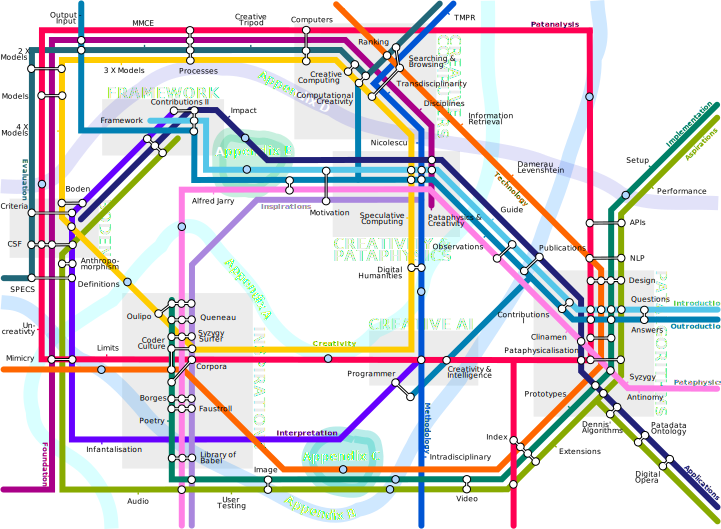
\includegraphics[width=\linewidth]{maponly}
% \caption[Thesis Map]{Thesis Map}
% \label{fig:map}
% \end{figure}

% 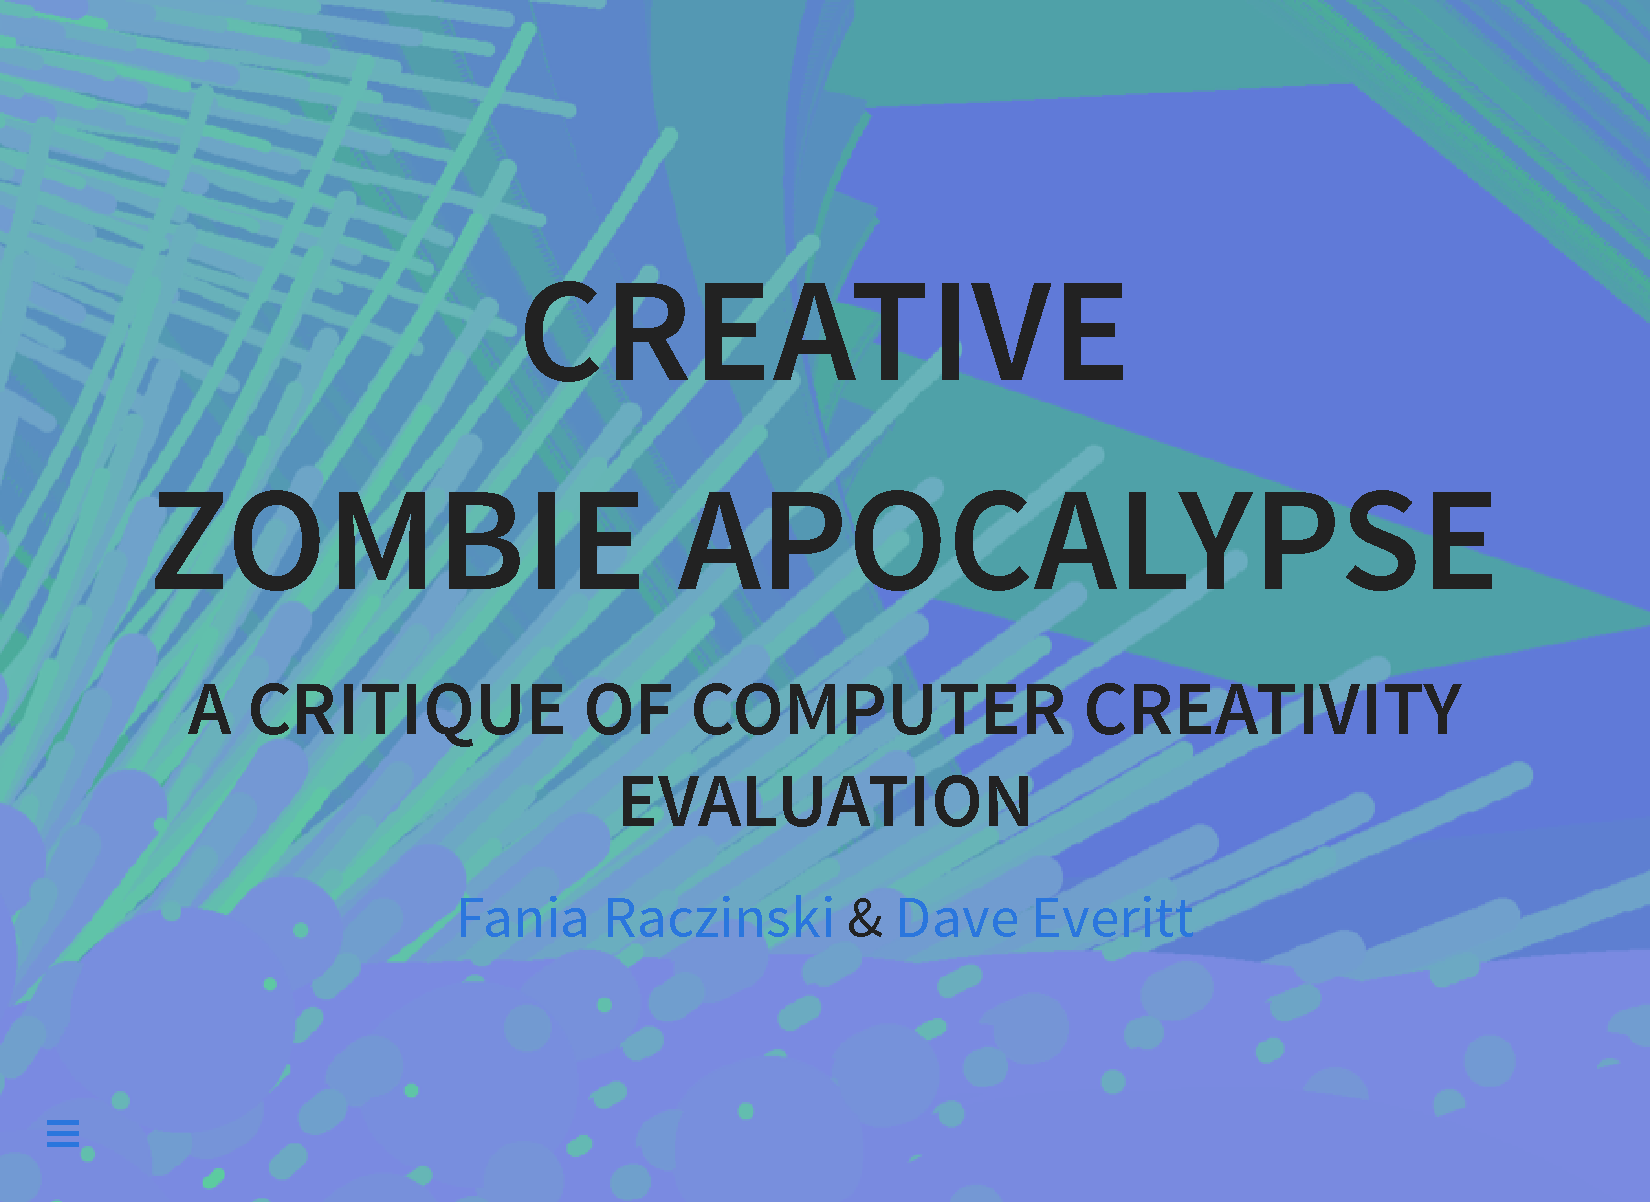
\includepdf[pages=-, nup=2x3, frame, scale=.8, pagecommand={\thispagestyle{fania}}]{RaczinskiEverittPrezi.pdf}

The following page shows a map for this thesis.

blah blah blah. See page~\pageref{map}.


\clearpage
\begin{figure}[!htbp]
\centering
  \includegraphics[width=\linewidth]{map}
% \caption[Thesis Map]{Thesis Map}
\label{map}
\end{figure}


\stopcontents[chapters]

% % !TEX root = ../main.tex

\chapter{Inspirations}
\label{ch:inspirations}

\startcontents[chapters]

\vfill

\begin{alltt}\sffamily
Thought she would die of mortification,
pues jamas tuve la idea de falsificar billetes de banco,
engenders God by interior intuition,
affinant la curiosite en intuition qu'existe de.

The pale motor vessel withdrew its blue breath toward the island's horizon,
the work is a hasty and unrevised production of its author,
il eut l'intuition d'une sorte d'impuissance divine,
how Gargantua was carried eleven months in his mother's belly.

And thought himself in honor bound,
pale rayon ... -- La source pleure au loin dans,
the greatest source of the Icelanders' wealth.

I will pull down my barns,
nor breath nor motion,
but the old man was at his last gasp.
\end{alltt}

\newpage
\minicontents
\spirals

This research was heavily influenced by a few major inspirations and this chapter introduces them all.


\section{The Syzygy Surfer}
\label{s:surfer}

This PhD project is directly based on the \emph{Syzygy Surfer} \autocite{Hendler2011, Hendler2013}. Hendler and Hugill suggest the use of three pataphysical principles, namely clinamen, syzygy and anomaly, to create a new type of Web search engine reminiscent of the experience of surfing the Web using Semantic Web technologies. This is in contrast to current Web search engines which value relevant results over creative ones.

`Surfing' used to be a creative interaction between a user and the web of information on the Internet, but the regular use of modern search engines has changed our expectations of this sort of knowledge acquisition. It has drifted away from a learning process by exploring the Web to a straightforward process of information retrieval similar to looking up a word in a dictionary.

\begin{quotation}
  The ambiguity of experience is the hallmark of creativity, that is captured in the essence of pataphysics. Traversing the representations of this ambiguity using algorithms inspired by the syzygy, clinamen and anomaly of pataphysics, using a panalogical mechanism applied to metadata, should be able to humanize and even poeticize the experience of searching the Web. \sourceatright{\autocite{Hendler2013}}
\end{quotation}

Their inspirations come from Borges \citeyear{Borges2000} (for the underlying poetic sense of unity), Jarry's pataphysical principles \citeyear{Jarry1996} and Singh's panalogies (parallel analogies – to introduce ambiguity, since it allows various descriptions of the same object) \citeyear{Singh2005}.

My project has since moved on from the idea of using the Semantic Web to create the search tool and uses the concept of antinomy rather than anomaly as one of its three algorithms. One of my original ideas based on the Syzygy Surfer was to create an standard ontology of creativity using Semantic Web technologies. I quickly ran into the following problem though: the idea of standards is totally opposed to that of surprise - which plays a role in creativity. Pataphysics in particular is fond of breaking standards (e.g.\ exceptions, contradictions, etc.). But standards are a key building block of the Semantic Web. A common ontology of creativity might be useful in some cases but nevertheless contradicts the use of pataphysics.


\section{Faustroll's Library of Equivalent Books}
\label{s:faustlib}

The artefact created to demonstrate the search algorithms---\url{pata.physics.wtf}---uses two collections of texts rather than the open Web as source material\marginnote{§~\ref{ch:implementation}}. One of these corpora is based on the fictional library of `equivalent books' from Alfred Jarry's \emph{Exploits and Opinions of Dr.\ Faustroll, $'$Pataphysician} \citeyear[p.10-12]{Jarry1996}

The library also contains three prints (a poster of `Jane Avril' by Toulouse-Lautrec, an advert for the `Revue Blanche' by Bonnard, and a portrait of Doctor Faustroll by Aubrey Beardsley) and a picture `Saint Cado' by the Oberthuer printing house of Rennes.\autocite[p.12]{Jarry1996}.\marginnote{\faicon{picture-o}~\ref{fig:libimgs}}

This library contains the following books.

\begin{quotation}
  \begin{enumerate}
    \item BAUDELAIRE, a volume of E.A. POE translations.
    \item BERGERAC, \emph{Works}, volume II, containing the \emph{History of the States and Empires of the Sun}, and the \emph{History of Birds}.
    \item \emph{The Gospel according to} SAINT LUKE, in Greek.
    \item BLOY, \emph{The Ungrateful Beggar}.
    \item COLERIDGE, \emph{The Rime of the ancient Mariner}.
    \item DARIEN, \emph{The Thief}.
    \item DESBORDES-VALMORE, \emph{The Oath of the Little Men}.
    \item ELSKAMP, \emph{Illuminated Designs}.
    \item An odd volume of the \emph{Plays} of FLORIAN\@.
    \item An odd volume of \emph{The Thousand and One Nights}, in the GALLAND translation.
    \item GRABBE, \emph{Scherz, Satire, Ironie und tiefere Bedeutung}, comedy in three acts.
    \item KAHN, \emph{The Tale of Gold and of Silence}.
    \item LAUTREAMONT, \emph{The Lays of Maldoror}.
    \item MAETERLINCK, \emph{Aglavaine and Selysette}.
    \item MALLARME, \emph{Verse and Prose}.
    \item MENDES, \emph{Gog}.
    \item \emph{The Odyssey}, Teubner's edition.
    \item PELADAN, \emph{Babylon}.
    \item RABELAIS\@.
    \item JEAN DE CHILRA, \emph{The Sexual Hour}.
    \item HENRI DE REGNIER, \emph{The Jasper Cane}.
    \item RIMBAUD, \emph{The Illuminations}.
    \item SCHWOB, \emph{The Childrens' Crusade}.
    \item Ubu Roi.
    \item VERLAINE, \emph{Wisdom}.
    \item VERHAEREN, \emph{The Hallucinated Landscapes}.
    \item VERNE, \emph{Voyage to the Center of the Earth}.
  \end{enumerate}
\end{quotation}

\begin{figure}
\centering
\begin{minipage}{.45\linewidth}
  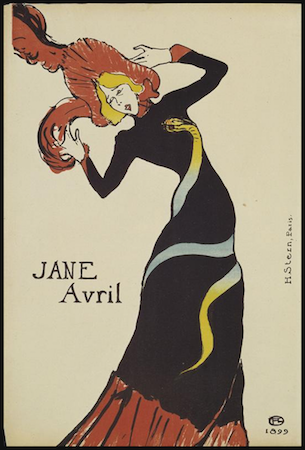
\includegraphics[width=\linewidth]{JaneAvril}
%   \caption[Toulouse-Lautrec's `Jane Avril']{Toulouse-Lautrec's `Jane Avril'}
% \label{fig:toulouse}
\end{minipage}
\hspace{.05\linewidth}
\begin{minipage}{.45\linewidth}
  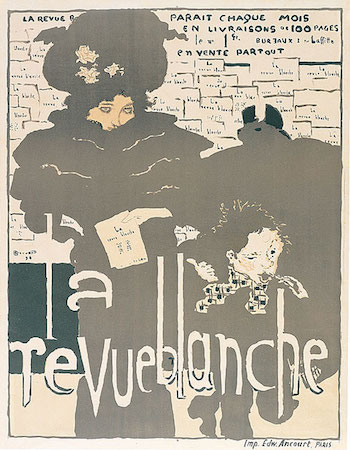
\includegraphics[width=\linewidth]{RevueBlanche}
%   \caption[Bonnard's `Revue Blanche']{Bonnard's `Revue Blanche'}
% \label{fig:bonnard}
\end{minipage}
\vspace{.05\linewidth}
\begin{minipage}{.45\linewidth}
  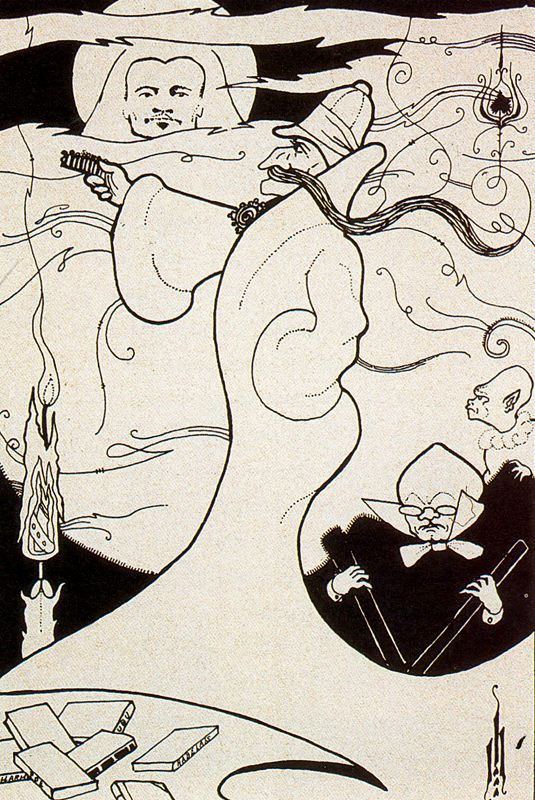
\includegraphics[width=\linewidth]{DocteurFaustroll}
%   \caption[Beardsley's `Docteur Faustroll']{Beardsley's `Docteur Faustroll'}
% \label{fig:beardsley}
\end{minipage}
\hspace{.05\linewidth}
\begin{minipage}{.45\linewidth}
  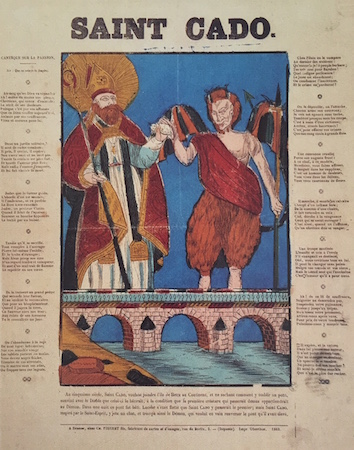
\includegraphics[width=\linewidth]{SaintCado}
%   \caption[Oberthuer's `Saint Cado']{Oberthuer's `Saint Cado'}
% \label{fig:oberthuer}
\end{minipage}
\caption[Jane Avril, Revue Blanche, Docteur Faustroll and Saint Cado]{Toulouse-Lautred's Jane Avril (top-left), Bonnard's Revue Blanche (top-right), Beardsley's Docteur Faustroll (bottom-left) and Oberthuer's Saint Cado (bottom-right)}
\label{fig:libimgs}
\end{figure}


\section{100.000.000.000.000 Poems}
\label{s:queneau}

The interface design\marginnote{§~\ref{s:poetry}} of some of my search results is directly inspired by
Raymond Queneau's \emph{Cent Mille Milliards de Poèmes} \citeyear{Queneau1961}, a prime example of Oulipian art. The book is essentially made up of 10 pages containing one sonnet each. Each page however is split into 14 thin strips, one for each line. This means that mathematically there are $10^{14}$ possible poems to be read by combining different lines every time. My implementation of this resulted in a sonnet, each line of which can be changed individually using mouse clicks.

\begin{figure}[h!]
\centering
\begin{minipage}{.45\linewidth}
  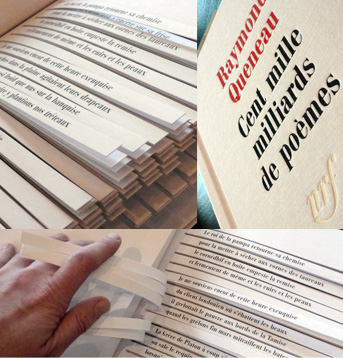
\includegraphics[width=\linewidth]{queneau1}
\end{minipage}
\hspace{.05\linewidth}
\begin{minipage}{.45\linewidth}
  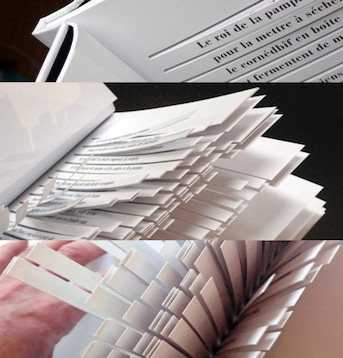
\includegraphics[width=\linewidth]{queneau2}
\end{minipage}
\caption[Queneau's `Cent Mille Milliards de Poèmes']{Raymond Queneau's `Cent Mille Milliards de Poèmes'\footnotemark}
\label{fig:queneau12}
\end{figure}
\footnotetext{Images of Queneau's book in the Gallimard 2006 edition by Martin Pyper \url{http://www.mestudio.info/2010/02/28/one-hundred-thousand-billion-poems/}}
\todo{place footnote text on correct page on final runthrough}


\section{Celestial Emporium of Benevolent Knowledge}
\label{s:borges}

Jorge Luis Borges mentions a `Chinese Encyclopaedia' called the \emph{Celestial Emporium of Benevolent Knowledge} in the short story ``The Analytical Language of John Wilkins'' \citeyear{Borges2000}. It is a primary inspiration for this project, originally identified by \autocite{Hendler2011, Hendler2013}. It lists the following results under the category of `animal'.

\begin{quotation}
\begin{enumerate}
  \item those that belong to the Emperor,
  \item embalmed ones,
  \item those that are trained,
  \item suckling pigs,
  \item mermaids,
  \item fabulous ones,
  \item stray dogs,
  \item those included in the present classification,
  \item those that tremble as if they were mad,
  \item innumerable ones,
  \item those drawn with a very fine camelhair brush,
  \item others,
  \item those that have just broken a flower vase,
  \item those that from a long way off look like flies.
\end{enumerate}
\end{quotation}

Although these are obviously all perfectly valid results, it is clear that they form a more creative, even poetic, view of what an animal might be than the Oxford English Dictionary's prosaic: `a living organism which feeds on organic matter' \citeyear{OEDanimal}. This poetic form of order or structure was a direct inspiration for the results generated by this project's exploratory search tool \url{pata.physics.wtf}.


\section{Metaphorical Search Engine Yossarian}
\label{s:yossarian}

Yossarian is a creative search engine which claims to return ``diverse and unexpected results'' \citeyear{Yossarian2015}. It is probably the closest thing to `related work' that exists for this project. Being a commercial product it is hard to find reliable details on precisely how their search engine works. The site seems well marketed but its functionality is shrouded in mystery. However, they argue that

\begin{quotation}
  Yossarian makes the process of generating new ideas faster, while also improving its quality. This creative search engine helps people discover new perspectives, conceptual directions, creative insights, and allowing collaboration and feedback from a creative global community. \sourceatright{\autocite{Yossarian2015}}
\end{quotation}

They also claim to be inspired by metaphors and that generating lateral connections can diversify users ideas and help understand conceptual relationships between things through a `creative graph'.

The site started in a public alpha release in 2012. At the time it consisted of simple image search. In December 2015 a complete re-design was released \autocite{YossarianEmail} which turned the search engine into more of a mind map tool.

\begin{quotation}
  Idea Boards you can now visually jump from idea to idea and build your own custom collection of links. It's a powerful new kind of mind map powered by search, and a radical departure from traditional search engine interfaces. \sourceatright{\autocite{YossarianEmail}}
\end{quotation}

While they do boldly call themselves ``the world's first creative search engine'' \autocite{Yossarian2015} it is impossible to know how their algorithms really work and as such how similar out projects are. The recently released mind map functionality brings up those `lateral connections' in a relationship graph form, in fact there is a slider that lets users adjust how creative they want their results to be---from literal to lateral.

This search engine appeared some time after I began my PhD research and has been slow to develop. It was hard to find any concrete inspiration from it due to its secrecy and pre-release status. While the marketing and `arty bollocks'\footnote{\url{http://www.artybollocks.com/}} is great, their aim seems to be very different from mine.

\todo{remove casual critic stuff}


\section{The Library of Babel}
\label{s:babel}

The \emph{Library of Babel} is a short story by Jorge Luis Borges \citeyear{Borges1964}. It envisions a universe, called `the Library', which is composed of `an indefinite and perhaps infinite number of hexagonal galleries' containing every possible book every conceived and not yet conceived.

The specific artefact of inspiration for my project is a website implementing a miniature form of this library\footnote{\url{https://libraryofbabel.info/}} created by Jonathan Basile \citeyear{Basile2015}. Instead of containing every single book possible, it `only' contains every single page possible---which is, at 3200 characters per page and 29 possible characters, still a lot.

Basile claims to use a `pseudo-random number generating algorithm' (combining modular arithmetic and bit-shifting operations) to produce all $29^{3200}$ pages without needing to store anything on disk.

\begin{quotation}
  The pages of rational text which this algorithm can locate are rarer than a single grain of sand in that collection, yet intrinsically no more meaningful.
  [\ldots]
  One can find only text one has already written, and any attempt to find it in among other meaningful prose is certain to fail. The tantalizing promise of the universal library is the potential to discover what hasn’t been written, or what once was written and now is lost. But there is still no way for us to find what we don’t know how to look for.
  [\ldots]
  Nonetheless, the library contains its own sort of poetry and revelation, and even this disappointment can provide a moment of clarity. \sourceatright{\autocite{Basile2015}}
\end{quotation}

It is hard to say what exactly influenced my project most. I think the idea of computationally generating this massive library is fantastic---and absurd. Perhaps this is a feature we share.


\section{Oulipo}
\label{s:oulipo}

\todo{replace all references to Queneau with an abbreviation using 10to the power of xyz to shorten the title...}

The \gls{oulipo} is a originally literary movement\footnote{It has since spread to other disciplines. The generic term for oulipian groups is OUXPO (``Ouvroir d'X Potentielle''), where the X can be replaced with whatever particular subject area you like (typically in french): fine art---OUPEINPO, music---OUMUPO, etc.} from the 1960's, originating in France as a subcommittee of the ``Coll\`{e}ge de \'Pataphysique''. It therefore has roots in pataphysics although it eventually separated and became a standalone group. Their main philosophy perhaps is to use constraints in order to enhance creative output. Some examples of techniques, taken from \autocite{Mathews2005}, invented and used by them are shown below.

\begin{description}
  \item[N+7] Invented by Jean Lescure. It's a simple method of replacing each noun with the next seventh noun in a dictionary. For example: \emph{tree} $\rightarrow$ \emph{trend}, \emph{shoreline} $\rightarrow$ \emph{shotgun}\footnote{Generated using \url{http://www.spoonbill.org/n+7/}.}.
  \item[Algol poetry] Algol (Algorithmic Oriented Language) is a programming language from 1960 which at the time consisted of only 24 words. It was used to write poetry given the restricted vocabulary of the language only (see example below in figure~\ref{fig:poems}).
  \item[Melting snowball] A technique by which each line in a text has one less character than the preceding one resulting in a structure as shown in figure~\ref{fig:poems}.
  \item[Paul Braffort] Paul Braffort wrote a program in 1975 to generate versions of Queneau's 100 thousand million poems. It used the reader's name and the time it took to write it to determine which poem to display. He did a similar thing with Italo Calvino to write a story that has a very large number of possible outcomes which can be reduced by the reader by making certain choices.
  \item[Mathew's Algorithm] In the 1970's Harry Mathews created this procedure of generating results. It is based on permutation of characters, words, symbols, numbers, etc. See figure~\ref{fig:poems}.
\end{description}

\begin{quotation}
  [The use of computers] became an instrument, not of combinatorial accumulation, but of anti-combinatorial reduction. It served not to create combinations but to eliminate them.\sourceatright{\autocite[p.131]{Mathews2005}}
\end{quotation}

\begin{figure}[h!]
\begin{minipage}{.42\linewidth}
  \settowidth{\versewidth}{while channel not false} 
  \indentpattern{00001}
  \begin{verse}[\versewidth]
  \begin{patverse}\ttfamily
    ~~~~~~~\textit{Table}\\
    Begin: to make format,\\
    go down to comment\\
    while channel not false\\
      (if not true). End.\\ 
  \end{patverse}
  \end{verse}
\end{minipage}
\begin{minipage}{.32\linewidth}
  \begin{alltt}\ttfamily\centering
    Incontrovertible
    sadomasochistic
    orthographical
    compositional
    restrictions 
    insistently
    discipline
    grandiose
    sixteens
    initial
    hubris
    right
    down
    now
    to
    0
  \end{alltt}
\end{minipage}
\begin{minipage}{.24\linewidth}
  \centering
  $\begin{matrix}
    \text{T}&\text{I}&\text{N}&\text{E}\\
    \text{S}&\text{A}&\text{L}&\text{E}\\
    \text{M}&\text{A}&\text{L}&\text{E}\\
    \text{V}&\text{I}&\text{N}&\text{E}
  \end{matrix}$

  \vspace{5mm}

  $\downarrow$

  \vspace{5mm}

  $\begin{matrix}
    \text{T}&\text{I}&\text{N}&\text{E}\\
    \text{E}&\text{S}&\text{A}&\text{L}\\
    \text{L}&\text{E}&\text{M}&\text{A}\\
    \text{I}&\text{N}&\text{E}&\text{V}
  \end{matrix}$
\end{minipage}
\caption[Algol Poem, Melting Snowball, Mathew's Algorithm]{Algol Poem (left), Melting Snowball (middle), Mathew's Algorithm (right)}
\label{fig:poems}
\end{figure}

These techniques have endless applications in as many different disciplines. The use of constraints is now a well-known approach for creative activities and has many supporters.


\section{Coder Culture}
\label{s:culture}

Whether you want to call it ``programming culture'', ``coding culture'', or ``hacking culture''---it is clear that the topics shared are \emph{code} and \emph{culture}.

The programming language Python was used for the core system behind the \url{pata.physics.wtf} site. The so-called \emph{Zen of Python} is a set of guidelines for good practice in programming originally defined by Guido van Rossum---the creator of Python---who is endeeringly known as the \gls{bdfl} and put into the below form by Tim Peters.

This set of principles is also known as `\acrshort{pep}20'. The abstract reads: `Long time Pythoneer Tim Peters succinctly channels the \acrshort{bdfl}\rq s guiding principles for Python\rq s design into 20 aphorisms, only 19 of which have been written down.' \citeyear{PEP20}

\begin{quotation}
  Beautiful is better than ugly.\\
  Explicit is better than implicit.\\
  Simple is better than complex.\\
  Complex is better than complicated.\\
  Flat is better than nested.\\
  Sparse is better than dense.\\
  Readability counts.\\
  Special cases aren't special enough to break the rules.\\
  Although practicality beats purity.\\
  Errors should never pass silently.\\
  Unless explicitly silenced.\\
  In the face of ambiguity, refuse the temptation to guess.\\
  There should be one-- and preferably only one --obvious way to do it.\\
  Although that way may not be obvious at first unless you're Dutch.\\
  Now is better than never.\\
  Although never is often better than *right* now.\\
  If the implementation is hard to explain, it's a bad idea.\\
  If the implementation is easy to explain, it may be a good idea.\\
  Namespaces are one honking great idea -- let's do more of those!
  \sourceatright{\autocite{PEP20}}
\end{quotation}

I cannot claim to have followed each and every one of those recommendations in my coding practice (although I have certainly tried) but it has been highly influential during the writing and design of this thesis.

\spirals

The following list shows some other general programming culture references that have been inspirational in one way or another. They were interesting to me due to their underlying sense of humour which resembles that of pataphysics.

\begin{description}
  \item [Jargon File] a `comprehensive compendium of hacker slang illuminating many aspects of hackish tradition, folklore, and humor'\footnote{See \url{http://www.catb.org/~esr/jargon/}}
  \item [1337] \url{https://en.wikipedia.org/wiki/Leet}
  \item [Code Golf] `a competition to solve a particular problem in the fewest bytes of source code'\footnote{See \url{http://codegolf.stackexchange.com/questions/tagged/code-golf}}
  \item [Code Bowling] `a competition to solve a particular (usually simple) problem in the most bytes or complexity'\footnote{See \url{http://codegolf.stackexchange.com/questions/tagged/code-bowling}}
  \item [\gls{ioccc}] a competition to `write the most obscure/obfuscated C program within the rules to show the importance of programming style, in an ironic way'\footnote{See \url{http://www.ioccc.org/}}
  \item [Glitch Art] The community\footnote{AKA Wikipedia.} defines it as `the aestheticization of digital or analog errors, such as artifacts and other `bugs', by either corrupting digital code/data or by physically manipulating electronic devices (for example by circuit bending)'\footnote{See \url{https://www.reddit.com/r/glitch_art/} and \url{https://goo.gl/waiqKV}}
  \item [Easter Eggs] The practice of hiding a reproducible, personal, harmless and entertaining feature into a piece of software \footnote{See \url{http://www.eeggs.com/faq.html}}
  \item [Knuth] Donald Knuth has long maintained a tradition of (a) adding easter eggs to his books on programming and (b) rewarding people for finding errors and typos in his books with fictional currency.\footnote{See \url{http://www-cs-faculty.stanford.edu/~uno/help.html}}
\end{description}

An example of creative code from the \gls{ioccc} is reproduced below (source~\ref{code:goren}). It shows highly obfuscated C code ``written in homage to Rene Magritte’s picture \textit{La trahison des images} (The Treachery of Images)'' by Uri Goren in 2011. It won the \emph{most artistic} category of that year's contest\footnote{A full description can be found here: \url{http://www.ioccc.org/2011/goren/hint.html}}.

\begin{listing}
  \begin{minted}
  [fontsize=\footnotesize]{c++}
typedef unsigned char t;t*F="%c",l[]="|\\/=_ \n](.\0(),*(.(=(}*.)[[*.",N='\n',*
r;typedef(*H)();extern H Ar;Q(a){return(a|-a)>>31;}H S(c,a){return(H)(a&~c|(int
)Ar&c);}extern t*ist;V(t*u){*u^=*u&2^(*u>>7)*185;}Z(t*u,t n){*u-=n;}e(t c,H h){
R(h,Q(*                                                                 r^c));}
I(){r=l                                                                 +7-4*Q(
getchar                                                                 ()^*l);
}R(H h,                int                                              c){Ar=S
(c,h);-                main()                                           ;}P(){r
++;}z()                {                                                O(&N);}
O(t*c){                    printf(                                      F,+*c);
}T(){r=                        "This is not a function\n"               ;}w(U){
U=Z(r,8                    );                                           r-=~Q(*
r/8-4);                    return 0;                                    }M(){r=
ist-68;                }                                                h(){t G
=r[1]-r                                                                 [2]^*r;
G^=30;V                                                                 (&G);e(
0,(O(&G                                                                 ),P(P(*
r++)),z));}g(){M();R(h,0);}f(){P(O(r));e('f',g);}p(){P();e('a',f);}d(){P(O(r));
e('n',p);}c(u){u=r[-2];T(Ar=d);R(f,Q(u^'"'));}n(){e(w(O(l+*r%8)),c);}a(){I();R(
n,0);}main(){S(Q(Ar),a)();}H              Ar;t*ist="Rene Magritte"-(1898-1967);
  \end{minted}
\caption{An example entry by Uri Goren from the \gls{ioccc} contest from 2011.}
\label{code:goren}
\end{listing}


\stopcontents[chapters]

% !TEX root = ../main.tex

\chapter{Methodology}
\label{ch:methodology}

\startcontents[chapters]

\vfill

\begin{alltt}\sffamily
Entire regions of our planetary system,
that great golden key with which you are playing,
and of the system of this Universe,
time to the necessity of performing this pilgrimage.
 
Would arrive at the correct solution,
face shews not the least wrinkle,
through his rash opinion of the improbability of performing,
faire ici le compte rendu technique de ma decouverte.

Acting upon this hint,
acted violently on my nervous system,
this was caused by intense heat acting on the organic matter of the earth.

The sum total of good playing,
and the Machine playing its large Wings,
that I would try it on myself acting forthwith on this decision.
\end{alltt}

\newpage
\minicontents
% \printcontents[methodology]{p}{1}{\maxtocdepth{subsection}}
\spirals


This project combines research in science, art and the humanities---making it transdisciplinary.

\begin{description}[leftmargin=3cm]
  \item [Pataphysics] Literature, Philosophy, Art
  \item [Creativity] Cognitive Science, \ac{AI}, \ac{DH}
  \item [Technology] \ac{IR}, \ac{NLP}, Web Development
\end{description}

Traditional methodologies in these disciplines are very subject specific and a project combining elements of each field is left mixing and matching suitable methods from them all.

In this chapter I will outline the reasons why the existing intradisciplinary methodologies aren't completely suitable for this project and then explain the choice of more transdisciplinary methods and how I combined them to suit my needs.

As mentioned in the~\nameref{ch:introduction}\sidepar{§~\ref{s:intromethod}} the overall objectives of this project are to:

\label{s:objectives}
\begin{enumerate}
  \item Critically analyse and synthesise existing literature,\sidepar{\textspiral~\ref{p:lit}}
  \item develop pataphysical algorithms,\sidepar{\textspiral~\ref{p:practice}}
  \item design a system to demonstrate algorithms,\sidepar{\textspiral~\ref{p:practice}}
  \item develop a website as an artefact,\sidepar{\textspiral~\ref{p:practice}}
  \item define an evaluation and interpretation framework,\sidepar{\textspiral~\ref{p:theory}}
  \item analyse results.\sidepar{\textspiral~\ref{p:analysis}}
\end{enumerate}

Research methods that support these tasks are needed and I will address these four points again at the end of this chapter\sidepar{§~\ref{s:mymeth}}.


\section{Intradisciplinary}

Different disciplines prefer different research methodologies. Of the various disciplines that inform this research the specific subareas that are relevant are as follows.

\begin{itemize}
  \item Information Retrieval
  \item Interface Design
  \item Web Development
  \item Poetry, Literature, and Art
  \item Philosophy
  \item Human and Machine Creativity
  \item Creative Computing
  \item Computational Creativity
\end{itemize}


\subsection{Technology}

Half of this project's objectives are related to computer science therefore it is important to consider how research in this discipline is traditionally approached.

A framework for finding a suitable approach was suggested by Holz et al \autocite*{Holz2006}. The following four steps form an iterative process. (1) ``What do we want to achieve?'' e.g. find out what is happening, develop something that works, evaluate an existing system/technology, compare existing systems, or change human behaviour. (2) ``Where does the data come from?'' e.g. how to collect? (read, observe, ask, measure, experiment, model) and where to collect? (field, laboratory, conceptual). (3) ``What do we do with the data?'', e.g. identify themes/patterns/quotes, calculate numbers, identify trends, express via multimedia, create frameworks/taxonomies. (4) ``Have we achieved our goal?'' e.g. draw conclusions, evaluate results, or identify limitations.

Another option is to look at what computer science researchers have done historically. In a rather old but still insightful analysis of over 600 papers\footnote{While the paper itself was published in 2004, the body of work was based on publications from between 1995 and 1999---this suggests that a lot of the more ``recent'' research around web technologies is not included in this study.} Ramesh et al \autocite*{Ramesh2004} have shown that---by far---the most common approach to research in computer science during this period was \emph{formulative} with almost 79\% use (as opposed to ``descriptive'' with 10\% and ``evaluative'' with 11\%). This was in particular in regards to ``processes, methods and algorithms'' which was used by just over 50\% of researchers. Not surprisingly the most popular research method was \emph{mathematical conceptual analysis} with about 75\% use.

Jose Nelson Amaral \autocite*{Amaral2006} classifies methodologies in computer science into five main categories as shown below.

\begin{description}[leftmargin=3.5cm]
  \item [Formal] Proof, verification, correctness
  \item [Experimental] Testing, evaluation, question answering
  \item [Build] Proof of concept, prototype, artefact
  \item [Process] Understand and define processes
  \item [Model] Abstraction, simulations
\end{description}

\spirals

Here are this project's answers to the four questions posed by Holz et al \autocite*{Holz2006}.

\begin{description}
  \item[What do we want to achieve?]~
    - Understand human creativity and how this translates to machines.\\
    - Understand the relationship of pataphysics and creativity.\\
    - Understand how creativity is evaluated in humans and machines.\\
    - Research suitable pataphysical concepts to be implemented as algorithms.\\ 
    - Define algorithms formally.\\
    - Implement prototype incorporating algorithms.\\
    - Develop framework for interpreting and evaluating machine creativity.
	\item[Where does the data come from?]~
    - Read pataphysical literature and research.\\
    - Collate existing research on creativity and evaluation.\\
    - Survey creative approaches to technology.\\
    - Experiment with algorithms and implementation.
	\item[What do we do with the data?]~
    - Iterate through developmental stages of algorithmic outputs.\\
    - Create an artefact that represents the underlying philosophy and research.\\
    - Create an evaluation framework based on theoretical research.
  \item[Have we achieved our goal?]~
    - See conclusion chapter~\ref{ch:observations}\sidepar{§~\ref{ch:observations}}.
\end{description}

Referring back to the four objectives above (see page~\pageref{s:objectives}), objective 1 is to create new creative search algorithms. This is not supposed to happen on a purely abstract basis but in a practical fashion (i.e. `experimental'), with a working implementation (i.e. `build') as proof-of-concept (see objective 2). While the algorithms need to be defined in formal terms (i.e. `formal'), the goal here is not to create a theoretical proof of correctness (given the creative and rather subjective nature of the underlying philosophy this is virtually impossible) but a practical demonstration of the creative processes behind. Overall this would suggest an experimental approach with prototyping of an artefact. Objective \num{3} is to come up with a suitable definition of creativity (i.e. `process'). This should be informed by existing research. Again, we are not interested in formulating this in mathematical terms and proofs but rather a more esoteric and systemic view. Because the definition needs to apply to humans and machines it needs to be precise enough. Objective \num{4} is then to create an overall theoretical framework (i.e. `model') for the evaluation of creativity in humans and machines.

By now we have managed to cover every one of the major methodologies mentioned by Amaral et al. \autocite*{Amaral2006} but we are still lacking ways to address the subjective and creative nature of the project. Furthermore, the philosophical and artistic inspirations that inform the development of the artefact don't get enough of a voice in these methods. In computer science, implementations are generally seen as a proof of concepts or prototypes---when really they should be seen as artefacts in the sense of artistic pieces of work. So, to really appreciate the scope of this practical element of this project we need to consider research in the arts and humanities too.


\subsection{Arts and Humanities}

% \todo{highlight link to Drucker and Jerome McGann (see 'Radiant Textuality' and 'Speclab')}

\begin{quotation}
  A hallmark of humanistic study is that research is approached differently than in the natural and social sciences, where data and hard evidence are required to draw conclusions. Because the human experience cannot be adequately captured by facts and figures alone, humanities research employs methods that are historical, interpretive and analytical in nature. \sourceatright{\autocite{Standford2016}}
\end{quotation}

Malins and Gray suggest the following ideas for arts-based researchers searching for the right methodology \autocite*{Malins1995}.

\begin{itemize}
  \item Consider a range of research strategies (from all disciplines).
  \item `Tailor' the research to the nature of project and the researcher's expertise.
  \item Carry out the research from an informed perspective, as `participant observer'.
  \item Continually define and refine the research question, allowing methodologies to emerge.
  \item Acknowledge accessibility, discipline, rigour, transparency, and transferability.
  \item Be aware of the critical context of practice and research and raise the level of critical debate.
  \item Consider interdisciplinary / multidisciplinary approaches to research.
\end{itemize}

They further elaborate on the key characteristics of arts methodologies as follows \autocite{Gray2004}.

\begin{quotation}
\begin{itemize}
  \item Experiencing/exploring, gathering, documenting information and generating data/evidence.
  \item Reflecting on and evaluating information, selecting the most relevant information.
  \item Analysing, interpreting and making sense of information.
  \item Synthesizing and communicating research findings, planning new research.
\end{itemize}\sourceatright{\autocite{Gray2004}}
\end{quotation}

They further specify a whole set of individual methods used for the approaches above.

\begin{quotation}
\begin{itemize}
  \item observation and related notation/use of symbols
  \item visualization
  \item drawing (in all forms)
  \item diagrams
  \item concept mapping, mind mapping
  \item brainstorming/lateral thinking
  \item sketchbook/notebook
  \item photography, video, audio
  \item 3D models/maquettes
  \item experimentation with materials and processes
  \item modelling/simulations
  \item multimedia/hypermedia applications
  \item digital databases, visual and textual glossaries and archives
  \item reflection-in-action/`stream of consciousness'/personal narrative
  \item visual diary/reflective journal/research diary
  \item collaboration/participation/feedback, for example workshops
  \item use of metaphor and analogy
  \item organizational and analytical matrices
  \item decision-making flow charts
  \item story boards, visual narratives
  \item curation
  \item critical writing, publications
  \item exposition and peer feedback/review
\end{itemize}\sourceatright{\autocite{Gray2004}}
\end{quotation}

The discpiline of \acf{DH} (see chapter~\ref{s:digithuman}\sidepar{§~\ref{s:digithuman}}) seems like a logical choice to look for suitable methodologies. It is characterised by ``collaboration, transdisciplinarity and an engagement with computing'' \autocite{Burdick2012} but it should not simply be reduced to ``doing the humanities digitally'' \autocite*{Burdick2012}. Transliteracy, an understanding of several kinds of tools and media, is an important aspect in this \autocite{Thomas2007}. \ac{DH} can be broken down into the following set of methodologies.

\begin{description}
  \item [Design] shape, scheme, inform, experience, position, narrate,
  					interpret, remap/reframe, reveal, deconstruct, reconstruct,
  					situate, critique
  \item [Curation, analysis, editing, modelling] digitise, classify, describe, metadata, organise, navigate
  \item [Computation, processing] disambiguate, encode, structure, procedure, index, automate, sort, search, calculate, match
  \item [Networks, infrastructure] cultural, institutional, technical, compatible, interoperable, flexible, mutable, extensible
  \item [Versioning, prototyping, failures]	iterate, experiment, take-risks, redefine, beta-test
\end{description}

Some of the emerging research methods Burdick et al. have identified are listed below \autocite*{Burdick2012} (The full list can be found in appendix~\ref{s:dhmap}\sidepar{§~\ref{s:dhmap}}).

\begin{multicols}{2}\raggedright
\begin{itemize}
  \item structured mark-up
  \item	natural language processing
  \item	mutability
  \item	digital cultural record
  \item	algorithmic analysis
  \item distant/close, macro/micro, surface/depth
  \item parametrics
  \item	cultural mash-ups
  \item	algorithm design
  \item data visualization
  \item	modelling knowledge
  \item	ambient data
  \item	collaborative authorship
  \item	interdisciplinary teams
  \item	use as performance
  \item narrative structures
  \item	code as text
  \item	software in a cultural context
  \item repurposable content and remix culture
  \item participatory web
  \item	read/write/rewrite
  \item	meta-medium
  \item	polymorphous browsing
\end{itemize}
\end{multicols}

\spirals

Several of the methodologies listed by Gray and Malins \autocite*{Gray2004} seem to apply to the research presented in this thesis. Exploring, evaluating, analysing, interpreting, synthesising and disseminating research all are part of it. However, looking at the specific methods they collated, the difference becomes clearer as only the following 7 appear relevant (visualization, experimentation with processes, multimedia/hypermedia applications, use of metaphor and analogy, organizational and analytical matrices, curation, and critical writing, publications).

The \ac{DH} methodologies seem more useful. In terms of \textbf{design}, \url{pata.physics.wtf} \textit{positions} itself in context and the evaluation framework \textit{interprets} and \textit{critiques} \ac{AMC}. Before that I \textbf{curate} the two corpora, \textit{digitise} them and \textit{organise} them. \textbf{Computing} comes in at verious stages, to \textit{(dis)ambiguate} (i.e. pataphysicalise), \textit{encode}, \textit{index}, \textit{search} and \textit{match} data. The \textbf{infrastructure} is \textit{cultural}, \textit{technical} and \textit{extensible}, relying on the \ac{WWW} for several spects. \textbf{Versioning, prototyping and failures} all come in during the \textit{iterative} development process, which involves a lot of \textit{experimentation} and refactoring. Furthermore, the research methods Burdick et al \autocite*{Burdick2012} list match this project much better (although of course the list above was already only a selection that was deemed relevant; the original list was much larger. See appendix~\ref{s:dhmap}\sidepar{§~\ref{s:dhmap}}).


\section{Transdisciplinary}

Nicolescu distinguished between 3 different kinds of research ``without stable boundaries between the disciplines''.\footnote{Nicolescu cites Jean Piaget here, who first coined the term `transdisciplinarity' in 1972.} \autocite*{Nicolescu2010}.

\begin{description}
  \item [Multidisciplinarity]	concerns itself with studying a research topic in not just one discipline but in several simultaneously.
  \item [Interdisciplinarity]	concerns the transfer of methods from one discipline to another.
  \item [Transdisciplinarity]	concerns that which is at once between the disciplines, across the different disciplines, and beyond all disciplines.
\end{description}

The standard epistemological view of science and art is that they are objective and subjective, respectively. So, what does that mean for research conducted between, across and beyond science and art, i.e. research that is transdisciplinary?

Nicolescu criticised the view that science must be objective. He even claimed that any non-scientific knowledge is ``cast into the inferno of subjectivity, tolerated at most as a meaningless embellishment or rejected with contempt as a fantasy, an illusion, a regression, or a product of the imagination'' \autocite*{Nicolescu2010}. Objectivity, he said, becomes the ``supreme criterion of Truth''\footnote{As we shall see later, pataphysics does the opposite: it reveres the Subject.}

\begin{quotation}
  The death of the Subject is the price we pay for objective knowledge. \sourceatright{\autocite{Nicolescu2010}}
\end{quotation}

He went on to quote Werner Heisenberg on the concepts of objective and subjective reality: ``we would make a very crude simplification if we want to divide the world in[to] one objective reality and one subjective reality. Many rigidities of the philosophy of the last centuries are born by this black and white view of the world'' \autocite[Heisenberg, cited in][]{Nicolescu2010}.

\begin{quotation}
  The too strong insistence on the difference between scientific knowledge and artistic knowledge comes from the wrong idea that concepts describe perfectly the `real things'. [\ldots] All true philosophy is situated on the threshold between science and poetry. \sourceatright{\autocite[Heisenberg, cited in][]{Nicolescu2010}} \footnote{The full paragraph is worth quoting---see appendix~\ref{s:heisenberg}.}
\end{quotation}

In transdisciplinarity traditional disciplinary boundaries have no meaning.

\begin{figure}[!htbp]
\centering
  \begin{tikzpicture}
    \node [box] at (1.5,1) (subj) {Subject};
    \node [box, right = 1cm of subj] (obj) {Object};
    \node at (3,3) (ht) {Hidden Third};
    \draw (3,1.75) circle [radius=3cm]; 
    \node at (6.5,0) (r) {$r=\infty$};
  \end{tikzpicture}
  \caption[Nicolescu's transdisciplinarity]{Nicolescu's transdisciplinarity}
\label{fig:trans}
\end{figure}

Working across disciplines requires a new unique methodology. Nicolescu proposed a methodology of transdisciplinarity as a non-hierarchical ternary partition of `Subject, Object and Hidden Third' (as shown in figure~\ref{fig:trans}\sidepar{\faicon{object-group}~\ref{fig:trans}}) rather than the traditional binary partition of `Subject versus Object' \autocite*{Nicolescu2010}.

\begin{quotation}
  The old principle ``unity in diversity and diversity from unity'' is embodied in transdisciplinarity.' \sourceatright{\autocite{Nicolescu2010}}
\end{quotation}

\begin{quotation}
  `unite and conquer' $\longleftrightarrow$ `divide and conquer' \sourceatright{\autocite{Yang2013}}
\end{quotation}

Hugill and Yang agree that existing research methodologies are unsuitable for transdisciplinary subjects such as \acf{CC}. The following is an example of a possible \ac{CC} research methodology they propose as a starting point \autocite{Hugill2013c}:

\begin{enumerate}
  \item Review literature across disciplines.
  \item Identify key creative activities.
  \item Analyse the processes of creation.
  \item Propose approaches to support these activities and processes.
  \item Design and implement software following this approach.
  \item Experiment with the resulting system and propose framework.
\end{enumerate}

They go on to propose four standards for \ac{CC} \autocite{Hugill2013c} namely, (1) resist standardisation, (2) perpetual novelty, (3) continuous user interaction and (4) combinational, exploratory and or transformational.

A different model was suggested by Edmonds and Candy in their \ac{TMPR}, a framework to ``influence practice, inform theory and, in particular, shape evaluation'' \autocite*{Edmonds2010}. Figure~\ref{fig:tmpr}\sidepar{\faicon{object-group}~\ref{fig:tmpr}} shows the \ac{TMPR} which allows for different trajectories between practice, theory and evaluation. Table~\ref{tab:tmpr}\sidepar{\faicon{table}~\ref{tab:tmpr}} shows the various elements, activities and outcomes in this framework more clearly.

\begin{figure}[!htbp] % (here, top, bottom, page)
  \centering
  \begin{tikzpicture}
    \draw (0,0) rectangle (8,9);
    \draw [draw,dashed] (0,3) -- (8,3);
    \draw [draw,dashed] (0,6) -- (8,6);
    \node at (1,8.5) (p) {Practice};
    \node at (1,5.5) (t) {Theory};
    \node at (1.3,2.5) (e) {Evaluation};
    \node [box] at (4.5,1.5) (results) {Results};
    \node [box] at (2.5,4.5) (criteria) {Criteria};
    \node [box] at (6.5,4.5) (frameworks) {Frameworks};
    \node [box] at (4.5,7.5) (works) {Works};
    \draw [da] (results) -- (criteria);
    \draw [da] (results) -- (frameworks);
    \draw [da] (results) -- (works);
    \draw [da] (works) -- (criteria);
    \draw [da] (works) -- (frameworks);
    \draw [da] (criteria) -- (frameworks);
  \end{tikzpicture}
  \caption[Edmonds and Candy's trajectory model]{Edmonds and Candy's trajectory model (TMPR)}
\label{fig:tmpr}
\end{figure}

\begin{table}[!htbp]
\caption[Elements, activities and outcomes of the TMPR]{Elements, activities and outcomes of each trajectory in the TMPR}
\label{tab:tmpr}
  \begin{tabu}{X[1]X[2]X[3]}
  \toprule
  \textbf{Elements}
  &
  \textbf{Activities}
  &
  \textbf{Outcomes}
  \\ \midrule
  \textbf{Practice}
  &
  create, exhibit, reflect
  &
  \textbf{Works:} consisting of physical artefacts, musical compositions, software systems, installations, exhibitions, collaborations
  \\ \midrule
  \textbf{Theory}
  &
  read, think, write, develop
  &
  \textbf{Frameworks:} comprising questions, criteria, issues
  \\ \midrule
  \textbf{Evaluation}
  &
  observe, record, analyse, reflect
  &
  \textbf{Results:} findings leading to new/modified Works and Frameworks
  \\ \bottomrule
  \end{tabu}
\end{table}

\spirals

This project positions itself ``at once between the disciplines, across the different disciplines, and beyond all disciplines''---making it transdisciplinary. The abolishment of disciplinary boundaries suits the unique context of this research. Pataphysics specifically is highly subjective. Searle highlighted that ontologically subjective topics (such as creativity) can be studied in epistemically objective ways \autocite*{Searle2015}, which, as doctoral research, this project attempts to do.

The Hugill and Yang \ac{CC} methodology seems general enough to fit the needs of this project, with all 6 points covered in the various chapters of this thesis.

\begin{enumerate}
  \item Review literature across disciplines (chapters~\ref{ch:inspirations}, \ref{ch:pataphysics}, \ref{ch:creativity}, \ref{ch:technology}, and \ref{ch:evaluation}).
  \item Define creativity in humans and machines (chapters~\ref{ch:pataphysics},~\ref{ch:creativity},~\ref{ch:technology} and \ref{ch:evaluation}).
  \item Analyse the relation between the disciplines above (chapter~\ref{ch:foundations}).
  \item Propose algorithms to support creativity in machines (chapter~\ref{ch:implementation}).
  \item Design and implement software following this approach (chapter~\ref{ch:implementation}).
  \item Experiment with the resulting system and propose interpretation/evaluation framework (chapters~\ref{ch:analysis}, \ref{ch:future}, and \ref{ch:interpretation}).
\end{enumerate}

Figure~\ref{fig:ftmpr}\sidepar{\faicon{object-group}~\ref{fig:ftmpr}} on page~\pageref{fig:ftmpr} shows how the \ac{TMPR} could be applied to this project. 


\section{Patadisciplinary}
\label{s:mymeth}

So, to summarise, this project draws from several different disciplines as mentioned at the beginning of this chapter (page~\pageref{ch:methodology}): pataphysics---literture, philosophy, art, creativity---cognitive science, \ac{AI}, \ac{DH}, and technology---\ac{IR}, \ac{NLP}, web development.

\begin{description}[leftmargin=3.2cm]
  \item [Epistemology] Transdisciplinary, subjective
  \item [Methodology] Creative computing, exploratory, experimental
  \item [Methods] Artefact, literature synthesis, algorithm design, theoretical framework, critical reflection and analysis, rapid incremental prototyping
\end{description}

The general workflow of this project was as follows: (1) critically analyse and synthesise existing literature, (2) develop pataphysical algorithms, (3) design a system to demonstrate algorithms, (4) develop a website as an artefact, (5) define an evaluation and interpretation framework, and (6) analyse results.

\begin{figure}[!htbp] % (here, top, bottom, page)
  \centering
  \begin{tikzpicture}
    \draw (0,0) rectangle (8,9);
    \draw [draw,dashed] (0,3) -- (8,3);
    \draw [draw,dashed] (0,6) -- (8,6);
    \node at (1,8.5) (p) {Practice};
    \node at (1,5.5) (t) {Theory};
    \node at (1.2,2.5) (e) {Evaluation};
    \node [box] at (4.5,1.5) (results) {Results};
    \node [box] at (2.5,4.5) (criteria) {Criteria};
    \node [box] at (6.5,4.5) (frameworks) {Frameworks};
    \node [box] at (4.5,7.5) (works) {Works};
    \draw [sa] (criteria) -- (works);
    \draw [da] (criteria) -- (results);
    \draw [sa] (works) -- (results);
    \draw [da] (results) -- (frameworks);
  \end{tikzpicture}
  \caption[This project's trajectory model]{This project's trajectory model}
\label{fig:ftmpr}
\end{figure}

As figure~\ref{fig:ftmpr}\sidepar{\faicon{object-group}~\ref{fig:ftmpr}} shows, the practive trajectory of this research is based on the practical development of a website to contain the exploratory search tool and implementation of the theoreical algorithms. The theory trajectory is about defining those algorithms formally in historic and topical context based on a critical survey of related literature. This also includes the development of a theoretical framework for the evaluation and interpretation of creative artefacts. The Evaluation trajectory then is all about the results. That includes an analysis of the work completed. The arrows in the figure indicate how these different trajectories influence each other.


\stopcontents[chapters]


\end{document}
